%*******************************************************************************
%****************************** Sixth Chapter *********************************
%*******************************************************************************

\chapter{ns-3 Implementation of LISP and LISP-MN}
\label{cha:ns-3}

% **************************** Define Graphics Path **************************
\ifpdf
    \graphicspath{{Chapter7/Pics/Raster/}{Chapter7/Pics/PDF/}{Chapter7/}}
\else
    \graphicspath{{Chapter7/Pics/Vector/}{Chapter7/}}
\fi

%-< ABSTRACT >--------------------------------------------------------------------
The \emph{Locator/Identifier Separation Protocol} (LISP) reconstructs the current IP addressing space so to be able to improve the no interrupt mobility issues. LISP Mobile Node (LISP-MN) is based on the basic LISP functionality to provide seamless mobility across networks. Thus, LISP can be implemented either on the border routers or directly on the end hosts to achieve the mobility. However, there are no experimental results comparing the advantages and disadvantages of each solution. The basic LISP architecture is deployed on LISP Beta Network and LISP-Lab platform to offer the researchers a realistic experimental environment, but both do not support LISP-MN. Some simulation models with LISP extensions are implemented on various simulators, but are not open source. Fortunately, there is an open source project implementing the fundamental LISP on ns-3 in 2016. Providing a free and flexible simulation model with the extensions so to help researchers quickly test new LISP mobility behaviors motivates our work. This chapter analyzes the different LISP mobility scenarios from the respects of handover delay and overhead of control plane. It describes the characteristics of each scenario. In addition, this chapter introduces the implementation of basic LISP architecture model and LISP-MN on the simulator ns-3. % It also provides the evaluation results in mobility scenario to validate the model and shows when the current proposal of LISP-MN is behind a LISP-site has a very high delay during the handover procedure.

The rest of chapter is organized as follows: Sec.~\ref{sec:ns3_related_work} introduces ns-3 and the existing LISP simulator on it. Sec.~\ref{sec:ns3_lispmn} analyzes the design and implementation of our prototype, and afterwards, Sec.~\ref{sec:ns3_analysis} illustrates three different LISP scenarios supporting seamless mobility, presents their traffic schema, modelizes the handover delay and overhead of control plane, and compares their advantages and disadvantages. % Sec.~\ref{sec:evaluation} presents preliminary evaluation results of our implementations. 
Sec.~\ref{sec:ns3_conclusion} provides some ideas of evaluation based on the proposed simulation for future work.
%-< ABSTRACT >--------------------------------------------------------------------

%-< SUB SECTION >--------------------------------------------------------------------
\section{Related work}
\label{sec:ns3_related_work}
 \subsection{Description of ns-3}
 \label{sec:ns3_ns3}
 ns-3~\cite{ns3} is a popular and free discrete-event network simulator for networking research. To be closer to the real implementation (in a real Operating System), easily include C-based implementation codes, ease debugging and reduce the cost on maintaining in a long term, C++ is prioritized to be the unique programming language for ns-3. Besides, ns-3 offers the possibility to visualize the simulation instance so to allow the users to visually confirm the packets flow as they expect.
%\begin{itemize}
%    \item Description of ns-3.
%    \item The simulator supporting LISP is introduced in Sec.~\ref{subsec:implementation_OMNet}.
%\end{itemize}

%-< SUB SECTION >--------------------------------------------------------------------
\subsection{Basic LISP implementation on ns-3}
\label{sec:ns3_basic_lisp}
It should be noted that this work is based on a prior implementation work by Lionel. However, his implementation has no support for LISP MN.


%-< SECTION >--------------------------------------------------------------------
\section{Implementation of LISP extensions on ns-3}
\label{sec:ns3_lispmn}

%-< FIGURE >--------------------------------------------------------------------
\begin{figure*}[!t]
	\centering
	\includegraphics[width=\textwidth]{Pics/LISP-NS3-UML}
	\caption{UML diagram of LISP/LISP-MN implementation. The solid arrow refers to a composition relation, while the blank one refers to a inheritance relation.}
	\label{LISP-UML}
\end{figure*}
%-< END FIGURE >--------------------------------------------------------------------
Our implementation is under ns-3.27 and based on LISP~\cite{rfc6830} and LISP-MN standards~\cite{meyer2016lisp}. The main classes are shown in Fig.~\ref{LISP-UML} in form of UML diagram. The blank blocks refer to the classes that we added into ns-3, while darker blocks are classes already in ns-3. As a design choice, we implement LISP/LISP-MN functionalities by modifying and extending the \emph{internet} module of ns-3, instead of creating a new independent module. The justification of this design is that LISP/LISP-MN and legacy internet module have an interdependent relationship. However, this kind mutually dependent relationship between modules is not supported by ns-3. Inspired from design of OpenLISP~\cite{saucez2009openlisp}, the Data Plane implementation is in "kernel space" (i.e. ns-3's \emph{TCP/IP stack}) and Control Plane is implemented in "user space" (i.e. ns-3 \emph{Application}). The communication between LISP Data and Control Plane is developed via a dedicated socket (i.e. \emph{LispMappingSocket}) that inherits from ns-3 \emph{Socket} class. It should be noted that our implementation only supports IPv4 at time of this writing. The IPv6 support (i.e. the implementation related to IPv6 such as \emph{LispOverIpv6Impl}) is still in process.  

%-< SUB SECTION >--------------------------------------------------------------------
\subsection{Implementation of LISP Data Plane}
\label{subsec:modifyInternet}
%\begin{itemize}
%    \item Modification of Receive method
%    \item Modification of Delivery method
%    \item Implementation of LISP encapsulation and decapsulation
%\end{itemize}
A LISP-compatible node (terminal or router) should be capable of determining whether a packet should be passed to LISP-related procedure and retrieving the associated mapping information if necessary. To this end, a new class called \emph{LispOverIp} and its extended classes (refer to Fig.~\ref{LISP-UML}) are added to ns-3 \emph{internet} module. This class is in charge of checking whether necessary to do LISP-related operations (\emph{NeedEncapsulation()}, \emph{NeedDecapsulation()}), and encapsulating conventional IP packets (i.e., \emph{LispOutput()}) as well as decapsulating LISP packets(\emph{LispInput()}). It also contains a smart pointer pointing to the LISP database and LISP cache. Both data structures (store the EID-RLOC mapping information) are represented by class \emph{SimpleMapTable} that inherits from \emph{MapTable}. The inheritanc mechanism allows other users to implement their own implementation of LISP database and cache. To support LISP functionalites, the \emph{Ipv4L3Protcol}, which is the IP layer implementation in ns-3, contains one \emph{LispOverIp} object and \emph{Ipv4L3Protcol}'s packet transmission and reception procedures are accordingly adapted.

To process outgoing packets, the adapted \emph{send()} in \emph{Ipv4L3Protcol} first verifies whether the \emph{LispOverIp} object is present. If yes, some checks are then conducted to determine that this packet should be processed by \emph{LispOutput()} (to encapsulate the packets) or by conventional packet transmission routine. For example, if both source and destination IP address of this packet belong to the same network, the LISP-related process (e.g., encapsulation) is skipped and this packet is processed as in a non-LISP network. Otherwise, EID-RLOC mapping information is searched from LISP cache and LISP database on LISP-MN node. In case of cache missing (i.e. destination RLOC is not found in the cache), the packet is dropped and \emph{SendNotifyMessage()} in \emph{LispOverIp} notifies the \emph{LispEtrItrApplication} that runs on LISP-MN node via a \emph{LispMappingSocket} socket. Once reception of cache missing event from LISP Data Plane (i.e. \emph{LispOverIp} object), \emph{LispEtrItrApplication} initiates a Map-Request message to LISP mapping system. Once reception of Map-Reply, the received EID-RLOC mapping is inserted into LISP cache. It should be noted that as an implementation choice, before the reception of Map-Reply message, all transmitted packets with the required RLOC as desination are dropped. One can also design a buffer to queue these packets and resend them once the required mapping informtion is received via Map-Reply. The advantage of such an implementation is to reduce the packet loss rate. 

For an incoming packet, if the destination of this packet is the node itself, the packet is processed by \emph{LocalDelivery} method in \emph{Ipv4L3Protocol}. Before passing to transport layer, \emph{LocalDelivery} checks if the packet should be decapsulated. If yes, it is passed to \emph{LispInput} method, in which the packet is decapsulated and reinjected in the IP stack. If the received packet destination is not this node, this packet is processed by patched \emph{IpForward} method. This packet may be ended up with LISP encapsulation procedure.

%-< SUB SECTION >--------------------------------------------------------------------
\subsection{Implementation of LISP Control Plane}
\label{subsec:control-plane-impl}
%\begin{itemize}
%    \item Implementation of xTR under ns3
%    \item Implementation of MS under ns3
%    \item Socket communication between control plan and data plan
%\end{itemize}
The implementation of LISP Control Plane at least should provide ITR/ETR, MR and MS. In practice, ETR and ITR functionalities are usually placed on a same router. In our implementation, they are included into classs \emph{LispEtrItrApplication}. A ns-3 node that runs \emph{LispEtrItrApplication} is a LISP-compatible router. It should be able to communicate with \emph{LispOverIp} on the same node (e.g. inform cache missing event) and other LISP-compatible routers (e.g. Map-Request/Map-Reply). To support LISP-MN feature, \emph{LispEtrItrApplication} also communicates with DHCP client application. For example, once a LISP-MN obtains an IP address from DHCP server, \emph{LispEtrItrApplication} receives the corresponding EID-RLOC mapping and sends a Map-Register message~\cite{meyer-lisp-mn-16}.

A node that runs a \emph{MapServer} application is the MS in a LISP-supported network. This class maintains a LISP database to store the EID-RLOC mapping information, learned from Map-Register message at the initialization stage. In current implementation, the role of MR is to receive the Map-Request message from xTR and forward it to the MS.

%-< SUB SECTION >--------------------------------------------------------------------
\subsection{Integration of TUN net interface card}
\label{subsec:tundevice}
To support mobility, LISP-MN actually can be regarded as a small LISP-Site, in which xTR functionalities and DHCP service are implemented, as well as configured address of MR and MS. As a LISP-MN node, it has a static permanent EID and dynamic RLOC assigned by the DHCP server. To differentiate with conventional RLOC of xTR interface, such kind of RLOC is referred to as the local RLOC (LRLOC). Different from conventional LISP node, at least two net interface cards (NIC) are installed into LISP-MN. One is \emph{WifiNetDevice}, the other is a TUN type card. The DHCP client application runs on LISP-MN's \emph{WifiNetDevice} and thus the LRLOC is allocated to this card. The permanent EID is assigned to \emph{VirtualNetDevice} net card. We modify the node's routing table so that each packet's inner header contains IP address on \emph{TunNetDevice} and outer header contains IP address of \emph{WifiNetDevice} as source address.

%-< SUB SECTION >--------------------------------------------------------------------
\subsection{Integration of DHCP}
\label{subsec:DHCP}
%\begin{itemize}
%    \item LISP-MN, in case of IPv4, need the intervention of DHCP procedure
%    \item The current version of DHCPv4 is not compatible with LISP
%    \item Implementation of LISP-compatible DHCPv4 based on conventional DHCPv4
%\end{itemize}
To support mobility within conventional LISP node, a modified DHCP client application is integrated into ns-3 node. To be compatible with LISP functionality, DHCP client application is modified. Once the DHCP client receives an allocated IP address (i.e. LRLOC), it notifies the \emph{LispEtrItrApplication} (i.e. LISP Control Plane) by sending a dedicated message that contains the EID-LRLOC mapping. \emph{LispEtrItrApplication} is in charge of populating the received mapping entry into LISP database. During the mobility process, when wireless link is down, the DHCP client flushes the LISP-MN database and populates the database again once reception of new LRLOC. 

% To support DHCP, conventional LISP-related process is also modified. For example, to transmit a DHCP Discovery message (application layer message), its source IP address is set as $0.0.0.0$. This message should be not processed by and should not passed to \emph{LispOutput} in \emph{LispOverIp}.


%-< SECTION >--------------------------------------------------------------------
\section{Theoretical analysis}
\label{sec:ns3_analysis}
As no matter LISP implemented on the border router or the end host can support seamless mobility, we design three different scenarios in this chapter to illustrate their characteristics, calculate their handover delay and overhead of control plane. 
%-< FIGURE >--------------------------------------------------------------------
\begin{figure}[!th]
	\centering
	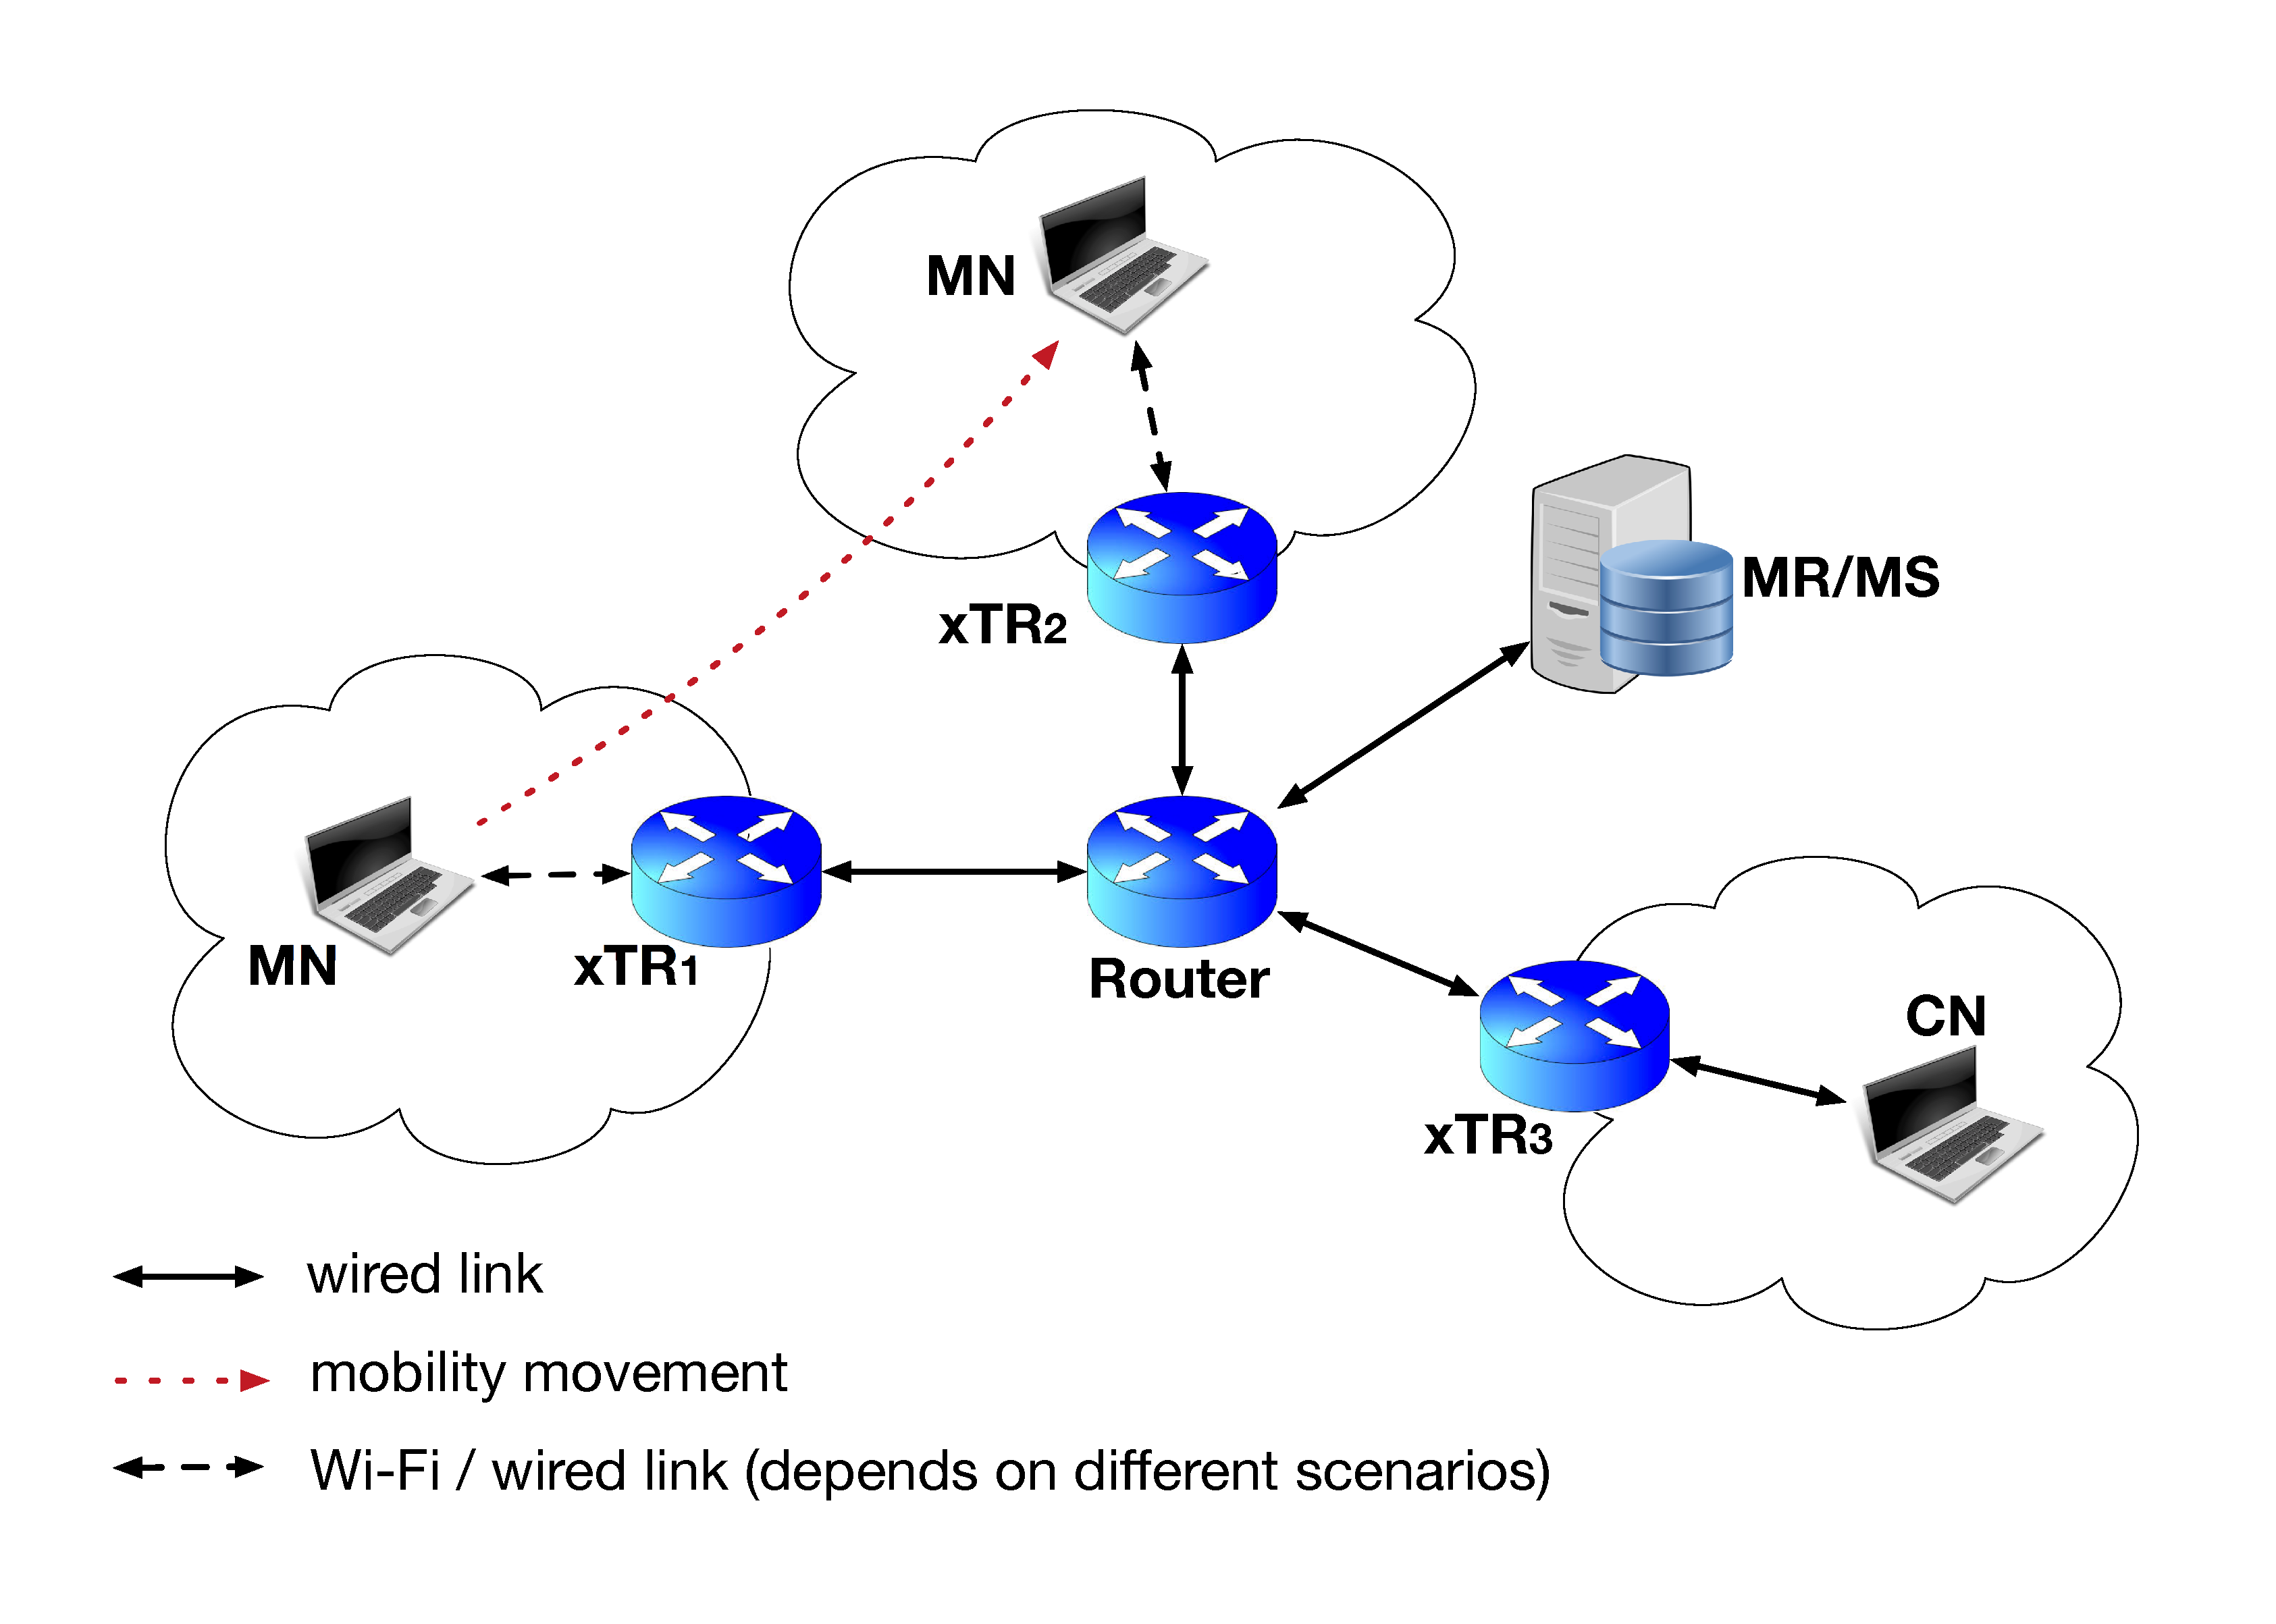
\includegraphics[width=0.8\textwidth]{Pics/LISP_mobility_archi}
	\caption{General scenario for LISP mobility architecture}
	\label{sim_archi}
\end{figure}
%-< END FIGURE >--------------------------------------------------------------------
\begin{enumerate}[noitemsep,topsep=0pt]
	\item The first scenario is LISP-MN in the non-LISP-Site (i.e., only the end host supports LISP). 
	\item The second one is MN in the LISP-Site (i.e., only the border router supports LISP). 
	\item The last scenario is LISP-MN in the LISP-Site (i.e., both the border router and the end host support LISP). 
\end{enumerate}	
% -<Descriptions with parameters>--------------------------------------------------------------------
% All the scenarios are based on a same simulation architecture shown in Fig.~\ref{sim_archi}, but with some slight differences, which will be respectively specified in the following parts from Sec.~\ref{sec:ns3_analysis_lispmn} to Sec.~\ref{sec:ns3_analysis_lispmn_xTR}. In our designed architecture, an MN is initially in the subnet of $Router_1$. An \emph{echo} application on MN sends packets to a remote stationary node CN in the LISP-Site of $xTR_3$. The distance between xTR\_1 and xTR\_2 is $170 m$. The connection between MN and xTR\_1 can be either Wi-Fi or wired link. If they use Wi-Fi, MN will move into the subnet of $Router_2$ at speed of $7.07 m/s$ after several seconds when the simulation begins. The start time of movement is a random value in the range of $[x, x] s$. At a certain moment during the moving, the Wi-Fi link between MN and $Router_1$ is down, which triggers the handover procedure. Afterwards, MN connects to $Router_2$ and reestablishes the communication with CN node. If they use wired link, the connection of MN with $Router_1$ will be down and the one with $Router_2$ will be up at the same time. This action also triggers the handover procedure. Every link between two network entities in this simulation architecture is set to $20 ms$.

All the scenarios are based on a same simulation architecture shown in Fig.~\ref{sim_archi}, but with some slight differences, which will be respectively specified in the following parts from Sec.~\ref{sec:ns3_analysis_lispmn} to Sec.~\ref{sec:ns3_analysis_lispmn_xTR}. In our designed architecture, an MN is initially in the subnet of $Router_1$. An \emph{echo} application on MN sends packets to a remote stationary node CN in the LISP-Site of $xTR_3$. The connection between MN and $Router_1$ can be either Wi-Fi or wired link. If they use Wi-Fi, MN will move into the subnet of $Router_2$ after several seconds when the simulation begins. At a certain moment during the moving, the Wi-Fi link between MN and $Router_1$ is down, which triggers the handover procedure. Afterwards, MN connects to $Router_2$ and reestablishes the communication with CN node. If they use wired link, the connection of MN with $Router_1$ will be down and the one with $Router_2$ will be up at the same time. This action also triggers the handover procedure.

In this chapter, we define the overall handover delay ($D_{overall}$) as the latency between the last packet received by MN from CN via $Router_1$ and the first packet received by MN from CN via $Router_2$ after the reestablishment. Same to the calculation of overall handover overhead ($C_{overall}$), which is the number of signals related to LISP control plane during that latency. According to the three following scenarios, the handover delay and overhead consist of different parts. All the necessary delay and LISP overhead of control plane during the mobility are listed in Tab.~\ref{Symbols_numerical_analysis}.
%-< TABLE >-----------------------------------------------------------------
\begin{table}[!tb]
	\centering
	\caption{Symbols for numerical analysis}
	\label{Symbols_numerical_analysis}{
		% \resizebox{0.9\textwidth}{!}{%
		\begin{tabular}{@{}|c|c|@{}}
			\hline\hline
			Symbols & Explanations   \\ \hline
			$D_{overall}$ & Overall handover delay	\\  \hline    
			$D_{DHCP}$ &  DHCP address configuration delay \\  \hline    
			$D_{Register}$ &  Delay of sending Map-Register      	\\  \hline
			$D_{Notify}$ &  Delay of receiving Map-Notify      	\\  \hline           
			$D_{Request}$ &  Delay of sending Map-Request to MDS      	\\  \hline   
			$D_{Reply}$ &  Delay of receiving Map-Reply      	\\  \hline      
			$D_{Resolve}$ &  Delay of resolving mapping information in MDS      	\\  \hline               
			$D_{SMR}$ &  Delay of sending SMR       	\\  \hline 
			$D_{invokeSMR}$ &  Delay of sending invoke-SMR \\  \hline 
			$D_{Link}$ &  Link delay between two network entities \\  \hline 
			$T_{A-B}$ &  Delay of packet transmission between A and B     	\\  \hline
			$T_{timeout_SMR}$ &  Timeout of SMR      	\\  \hline
			$C_{overall}$ &  Overall handover overhead \\  \hline    
			$C_{Register}$ &  Overhead of sending Map-Register      	\\  \hline
			$C_{Notify}$ &  Overhead of receiving Map-Notify      	\\  \hline           
			$C_{Request}$ &  Overhead of sending Map-Request to MDS      	\\  \hline   
			$C_{Reply}$ &  Overhead of receiving Map-Reply      	\\  \hline      
			$C_{SMR}$ &  Overhead of sending SMR       	\\  \hline 
			$C_{invokeSMR}$ &  Overhead of sending invoke-SMR \\  \hline  \hline    
		\end{tabular}
	}
\end{table}
%-< END TABLE >-----------------------------------------------------------------



%-< SUBSECTION >--------------------------------------------------------------------
\subsection{LISP-MN in non-LISP-Site}
\label{sec:ns3_analysis_lispmn}
The first scenario is the LISP-MN in non-LISP-Site, where the border routers are the conventional routers and LISP is only implemented on the mobile end host MN. In our simulation, the LISP-MN with permanent EID is initially placed in the subnet of $Router_1$, with the IP address distributed by $Router_1$ as its RLOC. The remote CN is a conventional stationary end host, residing in a LISP-Site of $xTR_3$. The LISP-MN communicates with CN by encapsulating the packets on itself and dencapsulating the packets on $xTR_3$, and the LISP-MN moves into subnet of $Router_2$ after the simulation begins. At a certain moment during the moving, the Wi-Fi link between LISP-MN and $Router_1$ is down, whereas LISP-MN detects $Router_2$, which triggers the handover procedure. LISP-MN first has a DHCP procedure with $Router_2$, so that the later distributes it a new IP address as its RLOC. Then LISP-MN needs register its new mapping information to the mapping system, and also send a $SMR$ to its communicating nodes in its cache (there is only $xTR_3$ in our scenario). $xTR_3$ sends an $Invoke SMR$ to the mapping system, so to obtain the new mapping information of LISP-MN. Afterwards, LISP-MN reestablishes the communication with CN node leveraging $Router_2$. The detailed traffic schema related to the handover procedure is indicated in Fig.~\ref{sim_schema_LISPMN}.  % The total simulation time is set to $45s$ and the DHCP procedure delay is set to $1s$. We conduct many times of simulations with the various beacon interval of Wi-Fi channel in the range of $0.05s$ to $2s$.
%-< FIGURE >--------------------------------------------------------------------
\begin{figure}[!th]
	\centering
	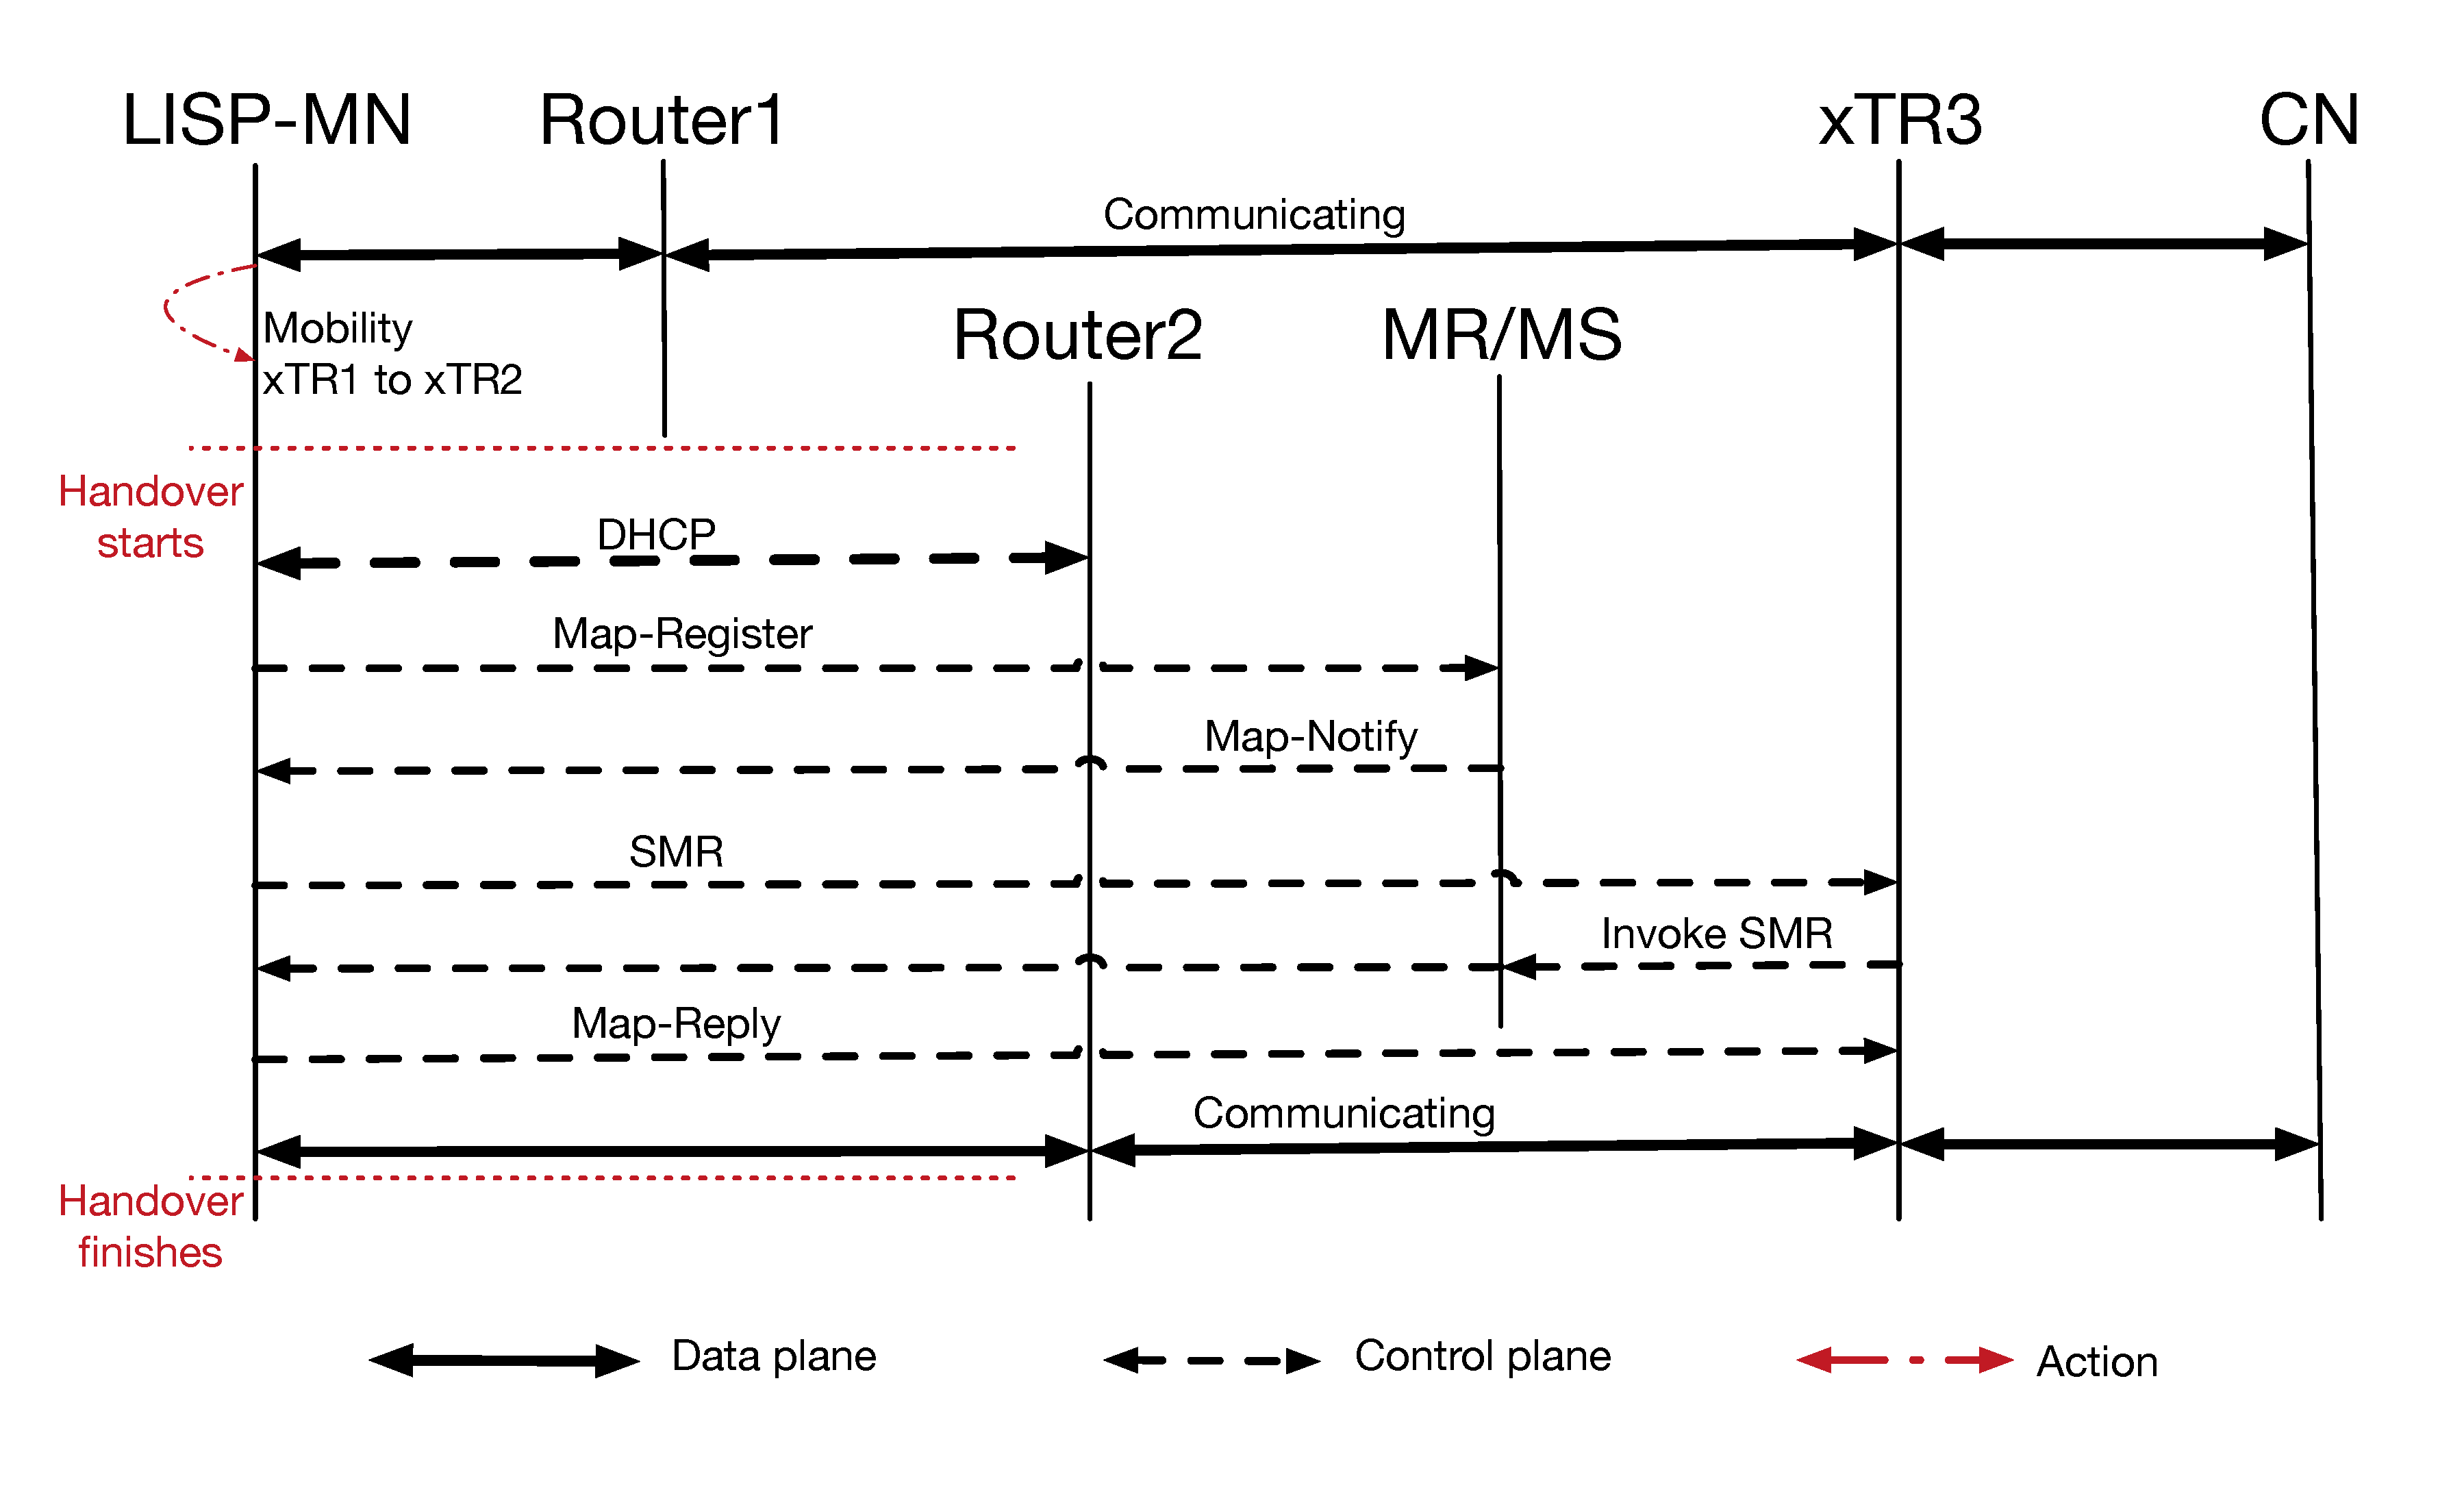
\includegraphics[width=0.8\textwidth]{Pics/Mobility_LISPMN_schema_SMR_simplify}
	\caption{Schema for LISP-MN mobility}
	\label{sim_schema_LISPMN}
\end{figure}
%-< END FIGURE >--------------------------------------------------------------------

The overall handover delay $D_{overall}$ in this scenario is composed by two parts: the DHCP related delay and LISP related delay. The delay of DHCP procedures consist of LISP-MN sending DHCP Discovery message to $Router_2$, receiving DHCP Offer message, sending DHCP Request message, and receiving DHCP ACK message. The delay of all the LISP procedures are presented in Fig.~\ref{sim_schema_LISPMN}. Thus, the overall handover delay is:
\begin{eqnarray}
D_{overall} &=& D_{DHCP} + D_{Register} + D_{Notify} + D_{SMR} + D_{invokeSMR} + D_{Reply} \nonumber \\
% &=& D_{DHCP} + T_{MN-MDS} + T_{MDS-MN} + T_{MN-xTR_3} + (T_{xTR_3-MDS} + D_{Resolve} + T_{MDS-MN}) + T_{MN-xTR_3} \nonumber \\
&=& D_{DHCP} + 3T_{MN-MDS} + 2T_{MN-xTR_3} + T_{xTR_3-MDS} + D_{Resolve} \nonumber \\
&=& D_{DHCP} + 3* (3*2ms) + 2*(3*2ms) + 2*2ms + 50ms\nonumber \\
&=& D_{DHCP} + 84 ms
\end{eqnarray}
where $D_{DHCP}$ represents the time elapsed between the DHCP Discover sent by the LISP-MN, and the $DHCP ACK$ message sent by the $Router_2$. Every link between two network entities in this simulation architecture is set to $2 ms$. % (Min value of handover delay = 1.073031 s, where packet sending interval = 0.01 s)

The overall handover overhead $C_{overall}$ includes the signaling overhead of registration when LISP-MN connects to $Router_2$, and the SMR procedure. Thus, the overall handover overhead related to LISP control plane is:
\begin{eqnarray}
C_{overall} &=& C_{Register} + C_{Notify} + C_{SMR} + C_{invokeSMR} + C_{Reply} \nonumber \\
&=& C_{Register} + C_{Notify} + C_{SMR} + 2C_{Request} + C_{Reply} \nonumber \\
&=& 6C
\end{eqnarray}

Adv\&Dis: Can achieve seamless handover through subnets. Not Slow.

Router is still normal router, can't help to reduce the BGP routing table size. EID needs permanent IP address.

%-< SUBSECTION >--------------------------------------------------------------------
\subsection{MN in LISP-Site}
\label{sec:ns3_analysis_xTR}
The second scenario is the MN in LISP-Site, where the mobile node MN is conventional and LISP are only implemented on the border routers. In our simulation, the MN is initially placed in the subnet of $xTR_1$, with the distributed IP address as its EID. The remote CN is same to the first scenario. The MN communicates with CN by encapsulating the packets on $xTR_1$ and dencapsulating the packets on $xTR_3$, and the MN moves into the coverage of $xTR_2$ after the simulation begins. Since the communication should not be interrupted during the mobility, this scenario limits the movement of MN being only within the same subnet, i.e., one of the EID-prefixes of $xTR_1$ is same to one of $xTR_2$'s. At a certain moment during the moving, the Wi-Fi link between MN and $xTR_1$ is down, whereas MN detects $xTR_2$, which triggers the switching connection procedure. Same to the first scenario, the DHCP procedure is necessary so to trigger the registration of new mapping information, but MN still keeps the former IP address as its EID, instead of $xTR_2$ distributing a new one to it. Then $xTR_2$ registers its new mapping information to the mapping system. As the mapping system find out that the EID of MN has been registered and associated by $xTR_1$, it sends a Map-Notify to both xTRs. The reason for sending to $xTR_2$ is the acknowledgment of the reception of its Map-Register. Whereas the purpose to $xTR_1$ is to tell it that the MN is now mapping with $xTR_2$ and inform the remote CN to update its mapping information. Since MN used $xTR_1$ to communicate with CN in the past time, only $xTR_1$ stored in its cache that to whom MN was exchanging the packets instead of $xTR_2$. Thus, $xTR_1$ sends a $SMR$ to $xTR_3$, and $xTR_3$ sends an $Invoke SMR$ to the mapping system, so to obtain the new mapping information of MN. Afterwards, MN reestablishes the communication with CN node leveraging $xTR_2$. The detailed traffic schema related to the handover procedure is indicated in Fig.~\ref{sim_schema_xTR}.
%-< FIGURE >--------------------------------------------------------------------
\begin{figure}[!th]
	\centering
	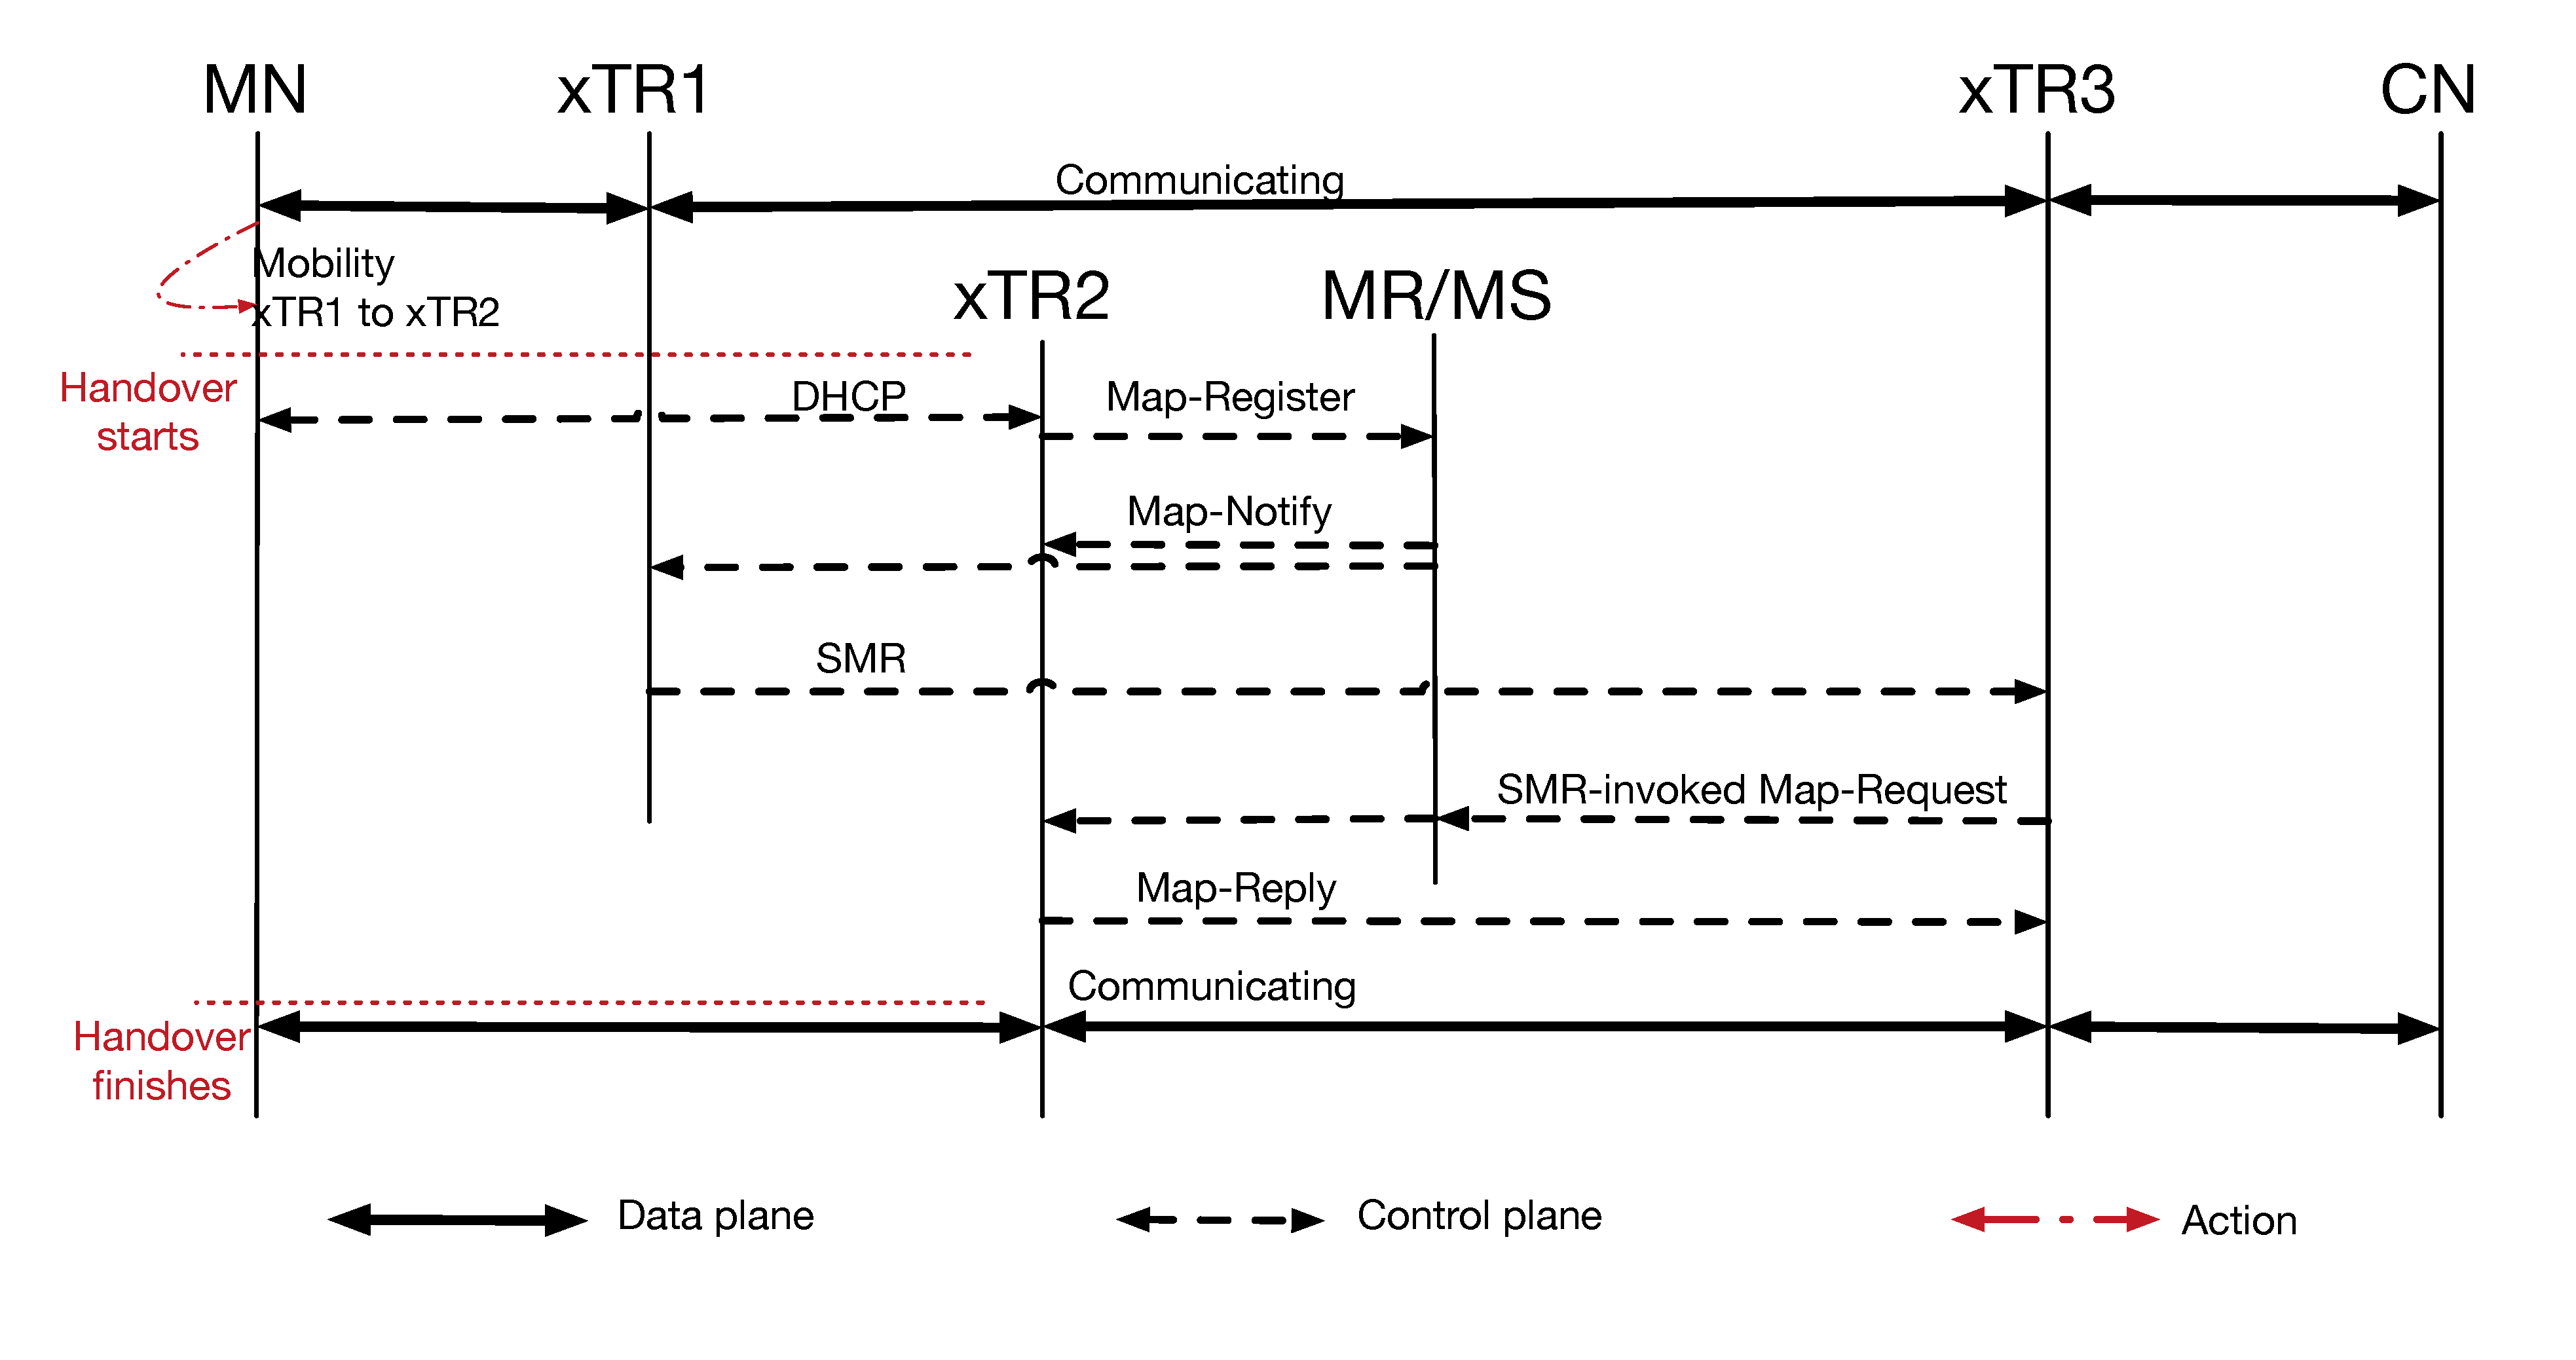
\includegraphics[width=0.8\textwidth]{Pics/Mobility_xTR_schema_SMR_simplify}
	\caption{Schema for LISP-MN mobility}
	\label{sim_schema_xTR}
\end{figure}
%-< END FIGURE >--------------------------------------------------------------------

The overall handover delay in this paper is defined at the moment that LISP-MN sending DHCP Discover message to xTR\_2 and end up with $xTR_3$ receiving the last Map-Reply from xTR\_2. Precisely, it is composed by three parts: the Wi-Fi association delay, the DHCP related delay and LISP SMR delay:
\begin{eqnarray}
D_{overall} &=& D_{DHCP} + D_{Register} + D_{Notify} + D_{SMR} + D_{invokeSMR} + D_{Reply} \nonumber \\
&=& D_{DHCP} +T_{xTR_2-MDS} + T_{MDS-xTR_1} + 3T_{xTR_1-xTR_3} \nonumber \\
&=& D_{DHCP} +2* (2*2ms) + 3*(2*2ms) \nonumber \\
&=& D_{DHCP} + 20 ms
\end{eqnarray}
where $D$ is the delay, $BI$ is Beacon Interval, subscriptions $Wi-Fi$, $DHCP$ and $SMR$ respectively refers to Wi-Fi association, DHCP procedure and LISP SMR. $CheckAlive$ is the delay that xTR\_1 checks if MN still connects to it. For example, xTR\_1 can simply \emph{ping} MN. If MN still connects to it, it will reply to mapping system that itself is still RLOC of MN. Otherwise, if \emph{ping} meets timeout, xTR\_1 will tell the mapping system that MN has left, and sends SMR to the CNs in its cache. The later situation has higher delay, because xTR\_1 needs to wait until timeout of \emph{ping}. (Min value of simulation = 1.067679 s, where includes 1 s of DHCP delay)

Adv\&Dis: Router is xTR, can help to reduce the BGP routing table size.

Can quickly achieve seamless switch the xTRs within a subnet, but can't through subnets.



%-< SUBSECTION >--------------------------------------------------------------------
\subsection{LISP-MN in LISP-Site}
\label{sec:ns3_analysis_lispmn_xTR}
Specify the architecture in this scenario.


%%-< SUB SECTION >--------------------------------------------------------------------
%\subsection{Simulation Setup}
%\label{subsec:ns3_setup_lispmn_xTR}
%%\begin{itemize}
%%    \item Topology of simulation setup
%%    \item The simulation parameter settings
%%\end{itemize}
%In our simulation, a LISP-MN with permanent EID 172.16.0.1 is initially placed in network 10.1.1.0/24. An \emph{echo} application on LISP-MN sends one packet per 0.01 second to a remote stationary node CN with EID 10.3.3.2, and the LISP-MN moves into network 10.1.7.0/24 at speed of $7.07m/s$. The distance between xTR\_1 and xTR\_2 is $170m$. LISP-MN node uses Wi-Fi to connect to xTR\_1. At a certain moment during the moving, the Wi-Fi link between LISP-MN and xTR\_1 is down, which triggers the handover procedure. Afterwards, LISP-MN connects to xTR\_2 and reestablishes the communication with CN node. The total simulation time is set to $45s$ and the DHCP procedure delay is set to $1s$. We conduct many times of simulations with the various beacon interval of Wi-Fi channel in the range of $0.05s$ to $2s$.

As shown in Fig.~\ref{sim_schema_LISPMN_xTR}, when MN sending the packets to CN during the simulation, it needs double encapsulation and the packet flow sequences are as follows. The traditional IP packets with EID 172.16.0.1 as source address and EID 10.3.3.2 as destination address are encapsulated by adding Local RLOC 10.1.1.1 as outer source address and RLOC 10.1.5.2 as outer destination address after MN querying the mapping information to MR. The LISP packets are encapsulated and forwarded to xTR\_1. The latter gets the mapping information from MR and encapsulates the packets again by adding the RLOC 10.1.2.1 as the outer source address and RLOC 10.1.5.2 as the outer destination address, then sends the packets on Internet core. The $xTR_3$ needs dencapsulate the packets twice after it receiving and verifying the packets, and finally sends to CN. Once LISP-MN lost its Wi-Fi connection with xTR\_1, it needs a DHCP procedure (consisting of DHCP Discover, DHCP Offer, DHCP Request and DHCP ACK) with xTR\_2 to get a new LRLOC 10.1.7.1 and then triggers LISP SMR to $xTR_3$. After $xTR_3$ getting new mapping information of <10.1.7.1, 10.1.3.1> and <172.16.0.1, 10.1.7.1>, the connection between LISP-MN and CN is re-established again.
%-< FIGURE >--------------------------------------------------------------------
\begin{figure}[!th]
	\centering
	\includegraphics[width=0.8\textwidth]{Pics/Mobility_double_encap_schema_SMR_simplify}
	\caption{Schema for LISP-MN in LISP-Site mobility}
	\label{Mobility_double_encap_schema_SMR_simplify}
\end{figure}
%-< END FIGURE >--------------------------------------------------------------------

The overall handover delay in this paper is defined at the moment that LISP-MN sending DHCP Discover message to xTR\_2 and end up with $xTR_3$ receiving the last Map-Reply from xTR\_2. Precisely, it is composed by three parts: the Wi-Fi association delay, the DHCP related delay and LISP SMR delay:
\begin{eqnarray}
D_{overall} &=& D_{DHCP} + D_{Register} + D_{Notify} + D_{SMR} + T_{timeout_SMR} + D_{SMR} + D_{invokeSMR} + D_{Reply} \nonumber \\
&=& D_{DHCP} + 2T_{LISPMN-MDS} + 4T_{LISPMN-xTR_3} + T_{timeout_SMR}\nonumber \\
&=& D_{DHCP} + 2* (3*2ms) + 4*(3*2ms) + 1s\nonumber \\
&=& D_{DHCP} + 1036 ms
\end{eqnarray}
During $T_{timeout\_SMR}$ (normally is 3 seconds), $xTR_3$ queries the mapping system for the RLOC of LISP-MN LRLOC.

%-< FIGURE >--------------------------------------------------------------------
\begin{figure}[!th]
	\centering
	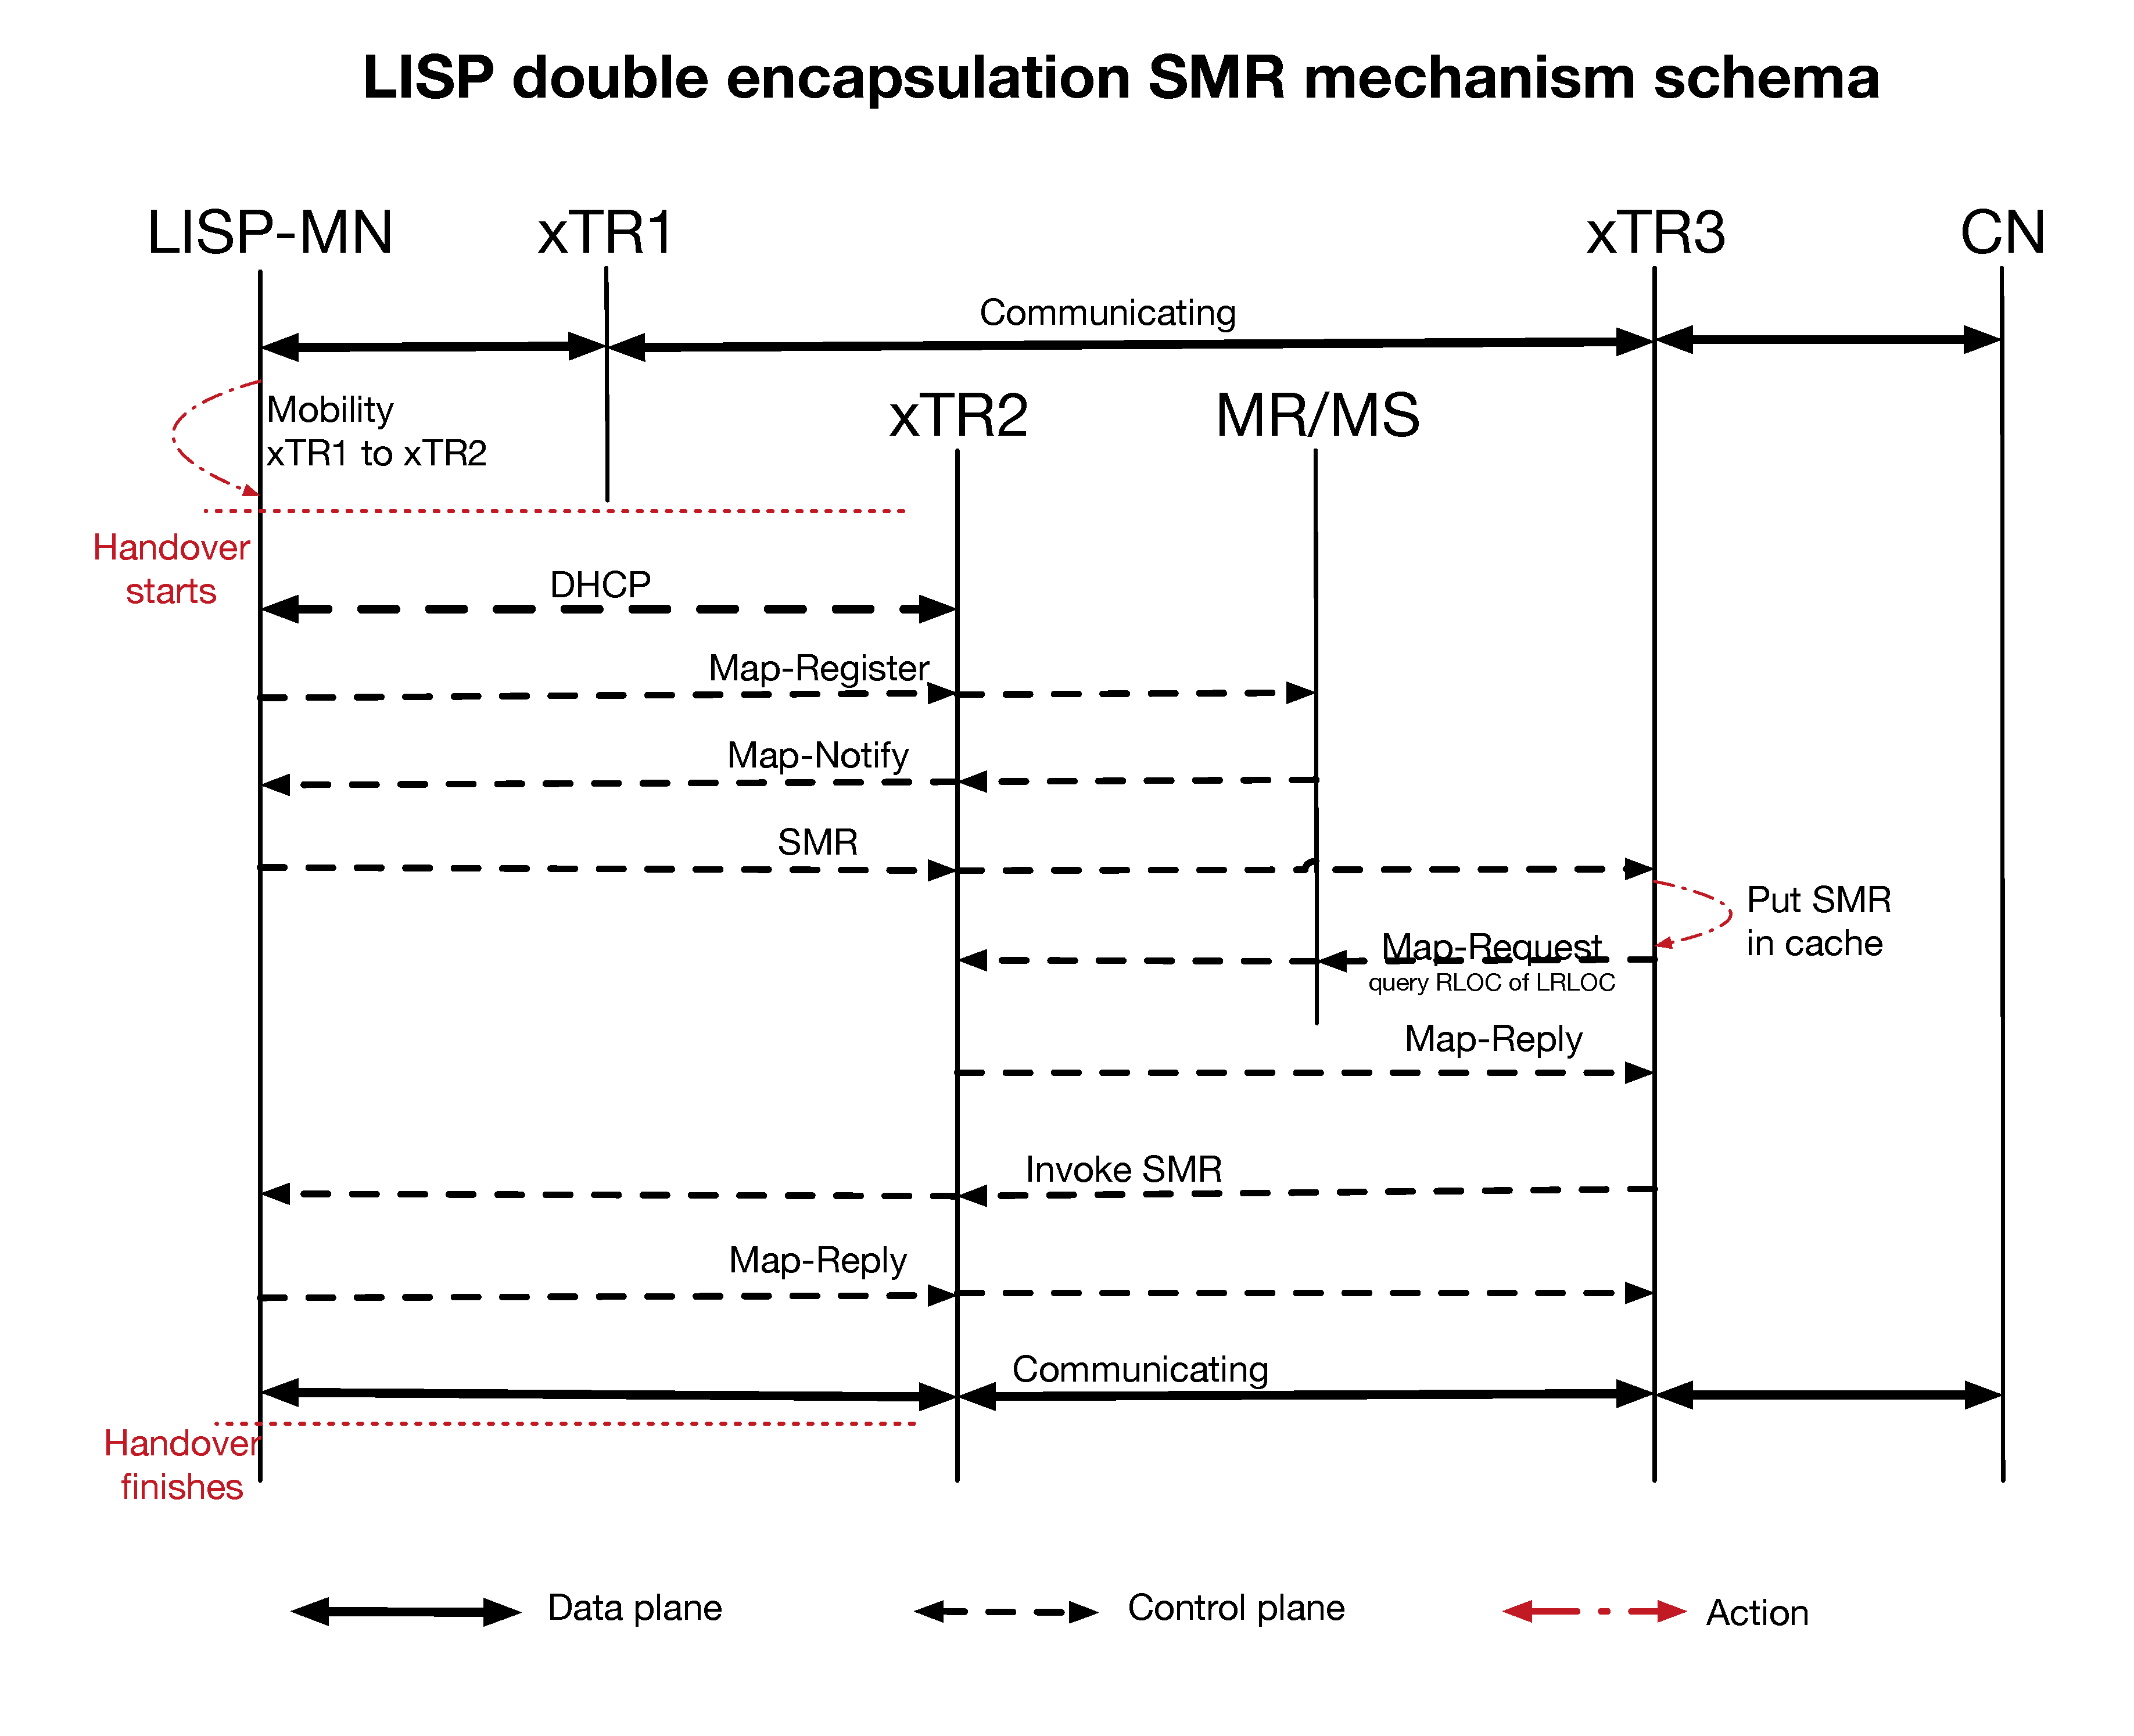
\includegraphics[width=0.8\textwidth]{Pics/Mobility_double_encap_schema_SMR_improving_simplify}
	\caption{Schema for LISP-MN in LISP-Site mobility}
	\label{Mobility_double_encap_schema_SMR_improving_simplify}
\end{figure}
%-< END FIGURE >--------------------------------------------------------------------
If we do not consider the security issues, the handover schema can be simplified as shown in Fig.~\ref{Mobility_double_encap_schema_SMR_improving_simplify}.
\begin{eqnarray}
	D_{overall} &=& D_{DHCP} + D_{Register} + D_{Notify} + D_{SMR} + D_{Request} + D_{Reply} + D_{invokeSMR} + D_{Reply} \nonumber \\
	&=& D_{DHCP} + 2T_{LISPMN-MDS} + D_{Resolve} + 3T_{LISPMN-xTR_3} \nonumber \\
	&=& D_{DHCP} + 2* (3*2ms) + 200ms + 3*(3*2ms) \nonumber \\
	&=& D_{DHCP} + 230 ms
\end{eqnarray}
where $D$ is the delay, $BI$ is Beacon Interval, subscriptions $Wi-Fi$, $DHCP$ and $SMR$ respectively refers to Wi-Fi association, DHCP procedure and LISP SMR. (Min value of handover delay = 1.300349, where packet sending interval = 0.02 s) 

After several executions of simulation program, we observe that the overall handover delay changes by the various beacon intervals, in particular the Wi-Fi association delay depends on the different beacon intervals, whereas LISP SMR procedure always cost around $3s$. To get the lower bound of overall handover delay, we can ignore the Wi-Fi association delay when the beacon interval is $500ms$, and the latency due to DHCP procedure is always $1s$. Thus, adopting LISP-MN to conduct the host-based mobility takes at least $4s$. Compared to current most stable solution for host-based IP mobility management MIPv6, which latency including L2 and L3 in a real Wi-Fi testbed is around $3.68s$~\cite{vassiliou2010analysis}, LISP-MN has a higher delay caused by the double encapsulation mechanism introduced by LISP-MN behind LISP-Site. 

During handover, CN can successfully receive packets from LISP-MN right after DHCP procedure being accomplished, but LISP-MN cannot receive the packets from CN until LISP SMR procedure is also finished. Thus, during DHCP procedure, all bi-directional transmitted packets are lost. To improve the performance, \cite{tang2017lisp} proposes a network-level LISP-MN solution, but has not validated their proposals neither in simulation nor in testbed. Our ns-3 implementation can be used to realize them.


Adv\&Dis: Router is xTR, can help to reduce the BGP routing table size. Can achieve seamless handover through subnets. EID needs permanent IP address.

Handover delay is longer than the other 2 mechanisms.







%%-< SECTION >--------------------------------------------------------------------
%\section{Evaluations}
%\label{sec:ns3_evaluation}
%%-< FIGURE >--------------------------------------------------------------------
%\begin{figure}[!th]
%	\centering
%	\includegraphics[width=0.7\textwidth]{Pics/LISP_mobility_LISPMN_PacketInterval}
%	\caption{Impact of packet sending interval on handover delay}
%	\label{LISP_mobility_LISPMN_PacketInterval}
%\end{figure}
%%-< END FIGURE >--------------------------------------------------------------------
%
%%-< FIGURE >--------------------------------------------------------------------
%\begin{figure}[!th]
%	\centering
%	\includegraphics[width=0.7\textwidth]{Pics/LISP_mobility_xTR_PacketInterval}
%	\caption{Impact of packet sending interval on handover delay}
%	\label{LISP_mobility_xTR_PacketInterval}
%\end{figure}
%%-< END FIGURE >--------------------------------------------------------------------
%
%%-< FIGURE >--------------------------------------------------------------------
%\begin{figure}[!th]
%	\centering
%	\includegraphics[width=0.7\textwidth]{Pics/LISP_mobility_double_encap_PacketInterval}
%	\caption{Impact of packet sending interval on handover delay}
%	\label{LISP_mobility_double_encap_PacketInterval}
%\end{figure}
%%-< END FIGURE >--------------------------------------------------------------------

%-< SECTION >--------------------------------------------------------------------
\section{Conclusion}
\label{sec:ns3_conclusion}
%\begin{itemize}
%    \item The validation of the implemented simulator
%    \item LISP-MN handover analysis
%    \item The potential of the implemented simulator
%\end{itemize}
As a promising technology for the future Internet architecture, LISP attracts more and more attention. There exist some LISP implementations, but they do not support LISP-MN or they are proprietary. Further, although measurements on LISP-testbeds can provide real time performance, due to the complicated topological structure, it is somewhat like a black box test which hinders us to find the exact explanation for some results. This highlights the importance to have an open source simulator for LISP in particular to support LISP-MN functionality. In this paper, we present our implementation for LISP/LISP-MN within ns-3, since the latter is a largely accepted simulator in networking research. The simulation results show that our implementation works well, and reveal the current LISP-MN proposal with a double encapsulation that has an high level delay during handover procedure. Our simulator can be a perfect choice to test the improvements of LISP-MN.

There are two possible directions to support IP mobility in LISP: host-based (i.e. LISP-MN) and network-based (i.e., xTR) mobility. We can compare the performance between LISP double encapsulation described in this paper with only host supporting LISP and only router supporting LISP leveraging our proposed simulator. As Map-Versioning~\cite{rfc6834} is another Mapping Cache update mechanism, we can also compare the performance between it and SMR that we present in this paper by our simulator.
